\documentclass[a4paper]{article}

\usepackage{inputenc}
\usepackage[british,UKenglish]{babel}
\usepackage{amsmath}
%\usepackage{titlesec}
\usepackage{color}
\usepackage{graphicx}
\usepackage{fancyref}
\usepackage{hyperref}
\usepackage{float}
\usepackage{scrextend}
\usepackage{setspace}
\usepackage{xargs}
\usepackage{multicol}
\usepackage{nameref}

\usepackage{sectsty}
\usepackage{multicol}
\usepackage{multirow}
\usepackage[procnames]{listings}
\usepackage{appendix}
\usepackage{listings}
\usepackage{caption}
\usepackage{multirow}

\usepackage{cite}
\bibliographystyle{IEEEtran}

\newcommand\tab[1][1cm]{\hspace*{#1}}
\hypersetup{colorlinks=true, linkcolor=black}
\interfootnotelinepenalty=10000

\newcommand{\cleancode}[1]{\begin{addmargin}[3em]{3em}\texttt{\textcolor{cleanOrange}{#1}}\end{addmargin}}
\newcommand{\cleanstyle}[1]{\text{\textcolor{cleanOrange}{\texttt{#1}}}}


\usepackage[colorinlistoftodos,prependcaption,textsize=footnotesize]{todonotes}
\newcommandx{\commred}[2][1=]{\textcolor{Red}
{\todo[linecolor=red,backgroundcolor=red!25,bordercolor=red,#1]{#2}}}
\newcommandx{\commblue}[2][1=]{\textcolor{Blue}
{\todo[linecolor=blue,backgroundcolor=blue!25,bordercolor=blue,#1]{#2}}}
\newcommandx{\commgreen}[2][1=]{\textcolor{OliveGreen}{\todo[linecolor=OliveGreen,backgroundcolor=OliveGreen!25,bordercolor=OliveGreen,#1]{#2}}}
\newcommandx{\commpurp}[2][1=]{\textcolor{Plum}{\todo[linecolor=Plum,backgroundcolor=Plum!25,bordercolor=Plum,#1]{#2}}}

\def\code#1{{\tt #1}}

\def\note#1{\noindent{\bf [Note: #1]}}

\makeatletter
%% The "\@seccntformat" command is an auxiliary command
%% (see pp. 26f. of 'The LaTeX Companion,' 2nd. ed.)
\def\@seccntformat#1{\@ifundefined{#1@cntformat}%
   {\csname the#1\endcsname\quad}  % default
   {\csname #1@cntformat\endcsname}% enable individual control
}
\let\oldappendix\appendix %% save current definition of \appendix
\renewcommand\appendix{%
    \oldappendix
    \newcommand{\section@cntformat}{\appendixname~\thesection\quad}
}
\makeatother




\lstset{frame=, basicstyle={\footnotesize\ttfamily}}



\graphicspath{ {images/} }
\usepackage{ctex}
\usepackage{listings}
\usepackage{multirow}
\usepackage{bm}
\usepackage{booktabs}
\usepackage{xcolor}

\colorlet{punct}{red!60!black}
\definecolor{background}{HTML}{EEEEEE}
\definecolor{delim}{RGB}{20,105,176}
\colorlet{numb}{magenta!60!black}

\lstdefinelanguage{json}{
    basicstyle=\normalfont\ttfamily,
    numbers=left,
    numberstyle=\scriptsize,
    stepnumber=1,
    numbersep=8pt,
    showstringspaces=false,
    breaklines=true,
    frame=lines,
    backgroundcolor=\color{background},
    literate=
     *{0}{{{\color{numb}0}}}{1}
      {1}{{{\color{numb}1}}}{1}
      {2}{{{\color{numb}2}}}{1}
      {3}{{{\color{numb}3}}}{1}
      {4}{{{\color{numb}4}}}{1}
      {5}{{{\color{numb}5}}}{1}
      {6}{{{\color{numb}6}}}{1}
      {7}{{{\color{numb}7}}}{1}
      {8}{{{\color{numb}8}}}{1}
      {9}{{{\color{numb}9}}}{1}
      {:}{{{\color{punct}{:}}}}{1}
      {,}{{{\color{punct}{,}}}}{1}
      {\{}{{{\color{delim}{\{}}}}{1}
      {\}}{{{\color{delim}{\}}}}}{1}
      {[}{{{\color{delim}{[}}}}{1}
      {]}{{{\color{delim}{]}}}}{1},
}

%-----------------------------------------BEGIN DOC----------------------------------------

\begin{document}
\renewcommand{\contentsname}{目\ 录}
\renewcommand{\appendixname}{附录}
\renewcommand{\appendixpagename}{附录}
\renewcommand{\refname}{参考文献} 
\renewcommand{\figurename}{图}
\renewcommand{\tablename}{表}
\renewcommand{\today}{\number\year 年 \number\month 月 \number\day 日}
\begin{titlepage}
\title{{\Huge \textbf{现代信息检索}{\large\linebreak\\}}{\Large \textbf{TREC Precision Medicine (PM) 2017}\linebreak\linebreak}}
%please write your name, Student #, and Class # in Authors, student ID, and class # respectively


\author{\\ \\ \\ \\ \\ \\ \\
\textbf{XXX 201818013229***}  \\ \\
\\ \\ \\ \\ \\ \\ \\  \\ \\ \\ \\ \\}

\date{\today}

\maketitle
\thispagestyle{empty}
\end{titlepage}


\newpage

\thispagestyle{empty}
\begin{center}
\tableofcontents\label{c}
\end{center}
\setcounter{page}{0}
\thispagestyle{empty}
\newpage

%------------------------------------------TEXT--------------------------------------------

%----------------------------------------OVERVIEW-----------------------------------------
\section{引言}

\subsection{任务}
对每个查询query,先在文档集中返回候选文档,再对其进行相关性排序,排序分值是0、1、2,分别代表不相关、相关和十分相关。评价指标使用的是P@5、P@10和P@15。

\subsection{数据集}
数据集使用的是clinical trials数据集:该数据集是由美国国家医学图书馆(U.S. National Library of Medicine)提供的资源,它包含了24万多的电子病历,每条病例包含简要的病人信息,包括疾病,基因,年龄,性别以及其它信息,有XML和TXT两个版本。其中,XML版本是官方集合,因为它具有每个摘要/试验的完整信息。TXT版本是为了便于处理,但不保证所有信息都包含在这些文件中。

\subsection{章节安排}
第一章为引言部分,对任务和数据集进行了简要的介绍。

第二章介绍了信息检索领域的相关工作。分别从检索模型、相关反馈和查询扩展、词嵌入以及深度神经网络这四个方面阐述了一些相关概念以及相关工作。

第三章对信息检索系统的搭建进行了详细的描述。包括索引的构建、对查询的扩展和所使用的检索模型。

第四章为文档重排部分。介绍了深度相关匹配模型(DRMM)的原理和架构,并分别说明了DRMM三个基本部分:匹配直方图映射、前馈匹配网络和词门控网络。

第五章是本文的实验部分。主要从实验设置和实验结果两方面展开介绍。其中,实验设置部分对实验步骤细节进行了详细的描述。实验结果部分展示并分析了本文设计的三大系统在测试集上的结果。

第六章为代码及运行方法说明。对本实验涉及到代码进行了解释并详细阐述了运行方法。

第七章总结并讨论了实验结果。其中,传统检索模型和深度匹配模型均取得了较好的结果。


\pagebreak
\section{相关调研} \label{relatedwork}%------------------------------
\subsection{检索模型}
信息检索模型是指如何对查询和文档进行表示,然后对他们进行相似度计算的框架和方法,本质上是对相关度建模。一个典型的检索模型通常由三部分组成:查询的表示、文档的表示、以及一个检索函数(基于查询和文档各自的表示,显式或隐式的估计两者相关的可能性)。

\subsubsection{布尔模型}
布尔模型是基于集合理论和布尔代数的一种简单的检索模型。它基于对特征项的严格匹配文本查询的匹配规则遵循布尔运算的法则。用户可以根据检索项在文档中的布尔逻辑关系提交查询,搜索引擎则根据事先建立的倒排文件结构,确定查询结果。标准的布尔逻辑模型为二元逻辑,所搜索的文档要么与查询相关,要么与查询无关。查询结果一般不进行相关性排序。

布尔模型的主要优点有两点:一是实现起来比较容易,速度快,计算的代价相对较少。二是查询语言表达简单,用户可以使用任意复杂的查询表达式,易于表示同义关系和词组。

它的缺点是,由于所有检索到的与用户查询条件相关的文档具有相同的检索状态值,则不能对查询结果按照相关性进行排序;另外关键词也没有考虑权重的影响,缺乏定量分析和灵活性以及不能表述模糊匹配。

\subsubsection{向量空间模型}
向量空间模型把信息库中的文本以及用户的查询都表示成向量空间中的点(向量),用它们之间夹角的余弦作为相似性度量,余弦距离越近,则相关性越大,最后根据相关性对搜索结果做排序。向量空间模型是现在的文本检索系统以及网络搜索引擎的基础。

向量空间模型的优点在于:1.检索词加权改进了检索效果。2.部分匹配策略允许检索出与查询条件相近的文献。3.可以根据相似度对文献进行排序。

它的缺点是,在这种模型中的基本假设,关键词Term向量之间被假设为相互无关的,而实际是有时它们之间大多是依赖关系,如在自然语言中,词或短语之间存在着十分密切的联系。所以这一假设对计算结果的可靠性造成一定的影响。另外,在查询中,也不能像布尔模型一样使用关键词之间的逻辑运算关系。

\subsubsection{概率模型}
概率模型主要是基于概率排序原则:即如果文档按照与查询的概率相关性的大小排序,那么排在最前面的是最有可能被获取的文档。它主要针对信息检索中相关性判断的不确定性以及查询信息表示的模糊性。在前面的向量模型中,我们假定关键词Term向量是正交的,不考虑Term向量之间的依赖关系。而在概率模型中,可以通过概率计算表达关键词Term之间,以及关键词Term和文档之间的依赖关系,预测文档与用户查询的相关概率,并可以对获取的结果按照相关度概率的大小进行排序(简称PRP)。

概率模型的主要缺点是对文本集的依赖性过强,而且条件概率值很难估计。概率模型的一个特例是贝叶斯网络,该网络以概率的方式定义了关键词的权重随着与其相关的关键词的权重的改变而改变方式。由于该模型适用于超文本信息系统,因而该模型的应用越来越广泛。但是该模型的缺点是,计算复杂度很大,因而该模型不适合很大的网络。

\subsection{相关反馈和查询扩展}
\subsubsection{相关反馈}
RF(relevance feedback,相关反馈)的主要思想是,在信息检索的过程中通过用户交互来提高最终的检索效果。

它的流程是:用户提交一个简短的查询后,系统返回初次检索结果,用户对部分结果进行标注,将它们标注为相关或不相关,之后系统基于用户的反馈计算出一个更好的查询来表示信息需求,并利用新查询系统返回新的检索结果。

相关反馈算法主要有Rocchio相关反馈算法和基于概率的相关反馈算法

相关反馈的评价的一个明显的策略就是,首先计算出原始查询的正确率—召回率曲线,一轮相关反馈之后,我们计算出修改后的查询 并再次计算出新的正确率—召回率曲线。也可以利用剩余文档集(residual collection,所有文档集中除去用户判定的相关文档后的文档集)对反馈后的结果进行评价。还可以给出两个文档集,一个用于初始查询和相关性判定,另一个用于比较和评价。

\subsubsection{查询扩展}
为了改善资讯检索召回率(Recall),而将原来查询句增加新的关键字来重新查询,此一技术称为扩展查询。搜索引擎会将使用者输入的查询句先做一次检索,根据检索出来的文件,选取出适合的关键字,加到查询句重新检索,借此来找出更多的相关文件。

它的方式有:使用人工编辑的一部受控词汇表;使用人工编纂的同义词词典;使用自动构建的同义词词典;基于查询日志挖掘进行查询重构。

此外,人工构建同义词词典的代价很大,一种取代思路是通过分析文档集来自动构造这种词典。这主要有两种实现方法。一种方法是简单地使用词共现信息。我们可以认为同时出现在文档或段落中的词在某种意义上相似或者相关,这样就可以通过计算文本中的统计信息来找到最相似的词。另一种方法是采用浅层语法分析器来分析文本得到词汇之间的语法关系或语法依存性。最简单的计算共现同义词词典的方法是基于词项之间的相似度计算。

\subsection{词嵌入}
词嵌入是自然语言处理(NLP)中语言模型与表征学习技术的统称。概念上而言,它是指把一个维数为所有词的数量的高维空间嵌入到一个维数低得多的连续向量空间中,每个单词或词组被映射为实数域上的向量。

词嵌入的方法包括人工神经网络、对词语同现矩阵降维、概率模型以及单词所在上下文的显式表示等。进行词嵌入后的词向量既能够降低维度,又能够捕捉到当前词在本句子中上下文的信息。

\subsection{深度神经网络}
\subsubsection{DSSM}
DSSM(Deep Structured Semantic Models)\cite{huang2013learning}是最早将深度模型应用在文本匹配的工作之一,该模型主要针对查询项和文档的匹配度进行建模,相对于传统文本匹配的模型,该方法有显著的提升。深度语义结构模型是典型的Siamese网络结构,每个文本对象都是由5层的网络单独进行向量化的,最后计算两个文本向量的余弦相似度来决定这两段文本的相似程度。

深度语义结构模型在文本向量化的时候分成了两个主要部分:第1部分是将文本中的每个单词,或者是由3个字母组成的片段做成一个最小单元,通过哈希方式映射到一个单词(字母片段)级别的向量,基于得到的单词向量,深度语义结构模型接上了3层的全连接来表达整个句子的主题向量,这个向量有128个维度。整个模型在训练的时候使用了大量的搜索系统的点击日志数
据,其中点击的作为正样本,并从没有点击的里面随机抽样一定量的负样本。然后正负样本组成一组,通过Softmax函数计算每个文档和查询项的匹配概率(加和为1),然后最大化所有正例的匹配概率的然函数。

\subsubsection{CDSSM}
微软的研究团队在成功提出深度语义结构模型之后,发现全连接的神经网络的参数太多,不利于优化,而且构造输入数据利用的是词袋模式,忽略了词
与词之间序的关系,对于匹配这种局部信息很强的任务,没法将一些学到的局部匹配信息应用到全局。于是进一步改进模型,提出了基于单词序列的卷积深度语义结构模型CDSSM (Convolutional Deep Semantic Model)\cite{shen2014learning}。卷积深度语义结构模型相对于深度语义结构模型,将中间生成句子向量的全连接层换成了卷积神经网络的卷积层和池化层,其它的结构和深
度语义结构模型是一样的。

卷积深度语义结构模型首先将查询项与文档中的每个单词(字母片段)都表示为一个词向量,然后对每个固定长度的窗口内的词向量进行卷积操作,得到针对这个窗口内短语的一个向量表达,之后卷积深度语义结构模型在这些卷积得到的向量上进行全局的池化操作,即对所有窗口输出的向量的相同位置取最大值。由于卷积的滑动窗口的结构形式考虑到了句子中的单词顺序信息,在相关度判断的准确度方面相对于深度语义结构模型有了一定的提升。

\subsubsection{ARC-I}
华为诺亚方舟实验室的李航等人参考在文本分类任务中kim提出的卷积神经
网络来建模句子表达的思想,提出上午ARC-I模型\cite{hu2014convolutional}也使用了卷积神经网络的结构来进行文本匹配。ARC-I直接将两个待匹配的句子表达为两个定长的向量,然后拼接两个向量并输入一个全连接的多层神经网络,从神经网络的输出得到最终的匹配。

\subsubsection{MatchPyramid}
MatchPyramid\cite{pang2016study}主要方法是构建文本与文本的相似矩阵,采用CNN对矩阵进行打分,分数越高的值对应的文本与文本直接相关性越高。 算法架构是输入两个文本,基于glove得到两文本的每个词的embedding,然后构建两个文本的相似矩阵,并把相似矩阵放入两层CNN中,把CNN的结果放入两层的感知机中,最后获得二分类的score。

\subsubsection{DRMM}
DRMM(deep relevance matching model)\cite{guo2016deep}主要用于问答相关的长短文本匹配,在进行匹配之前,先对问题文本即短文本进行重构,把embed的向量重构之后得到文本新的表征,再进行匹配。 
%------------------------------
\pagebreak

\section{信息检索}
我们首先从clinical trials数据集中提取数据,利用ElasticSearch建立索引,搭建初步的信息检索系统。
\subsection{索引}
我们使用ElasticSearch\footnote{https://www.elastic.co}来索引clinical trials. ElasticSearch是一个分布式的搜索和分析引擎,可以用于全文检索、结构化检索和分析,并能将这三者结合起来。ElasticSearch 基于 Lucene开发,现在是使用最广的开源搜索引擎之一,Wikipedia、Stack Overflow、GitHub 等都基于 ElasticSearch 来构建他们的搜索引擎。

索引的字段有:brief\_title、official\_title、brief\_summary、detailed\_des-cription、overall\_status、condition、eligibility、gender、gender\_based、minimum\_age、maximum\_age、keyword、mesh\_term。这些字段对应clinical trials数据集中XML文档中的XML元素标签。

\subsection{查询扩展}
在许多文档集中,同一概念可以用不同的词来表达,如“Colonic Neoplasm”和“Cancers, Colon”具有相同的含义,这个现象称为一词多义,这种现象会对信息检索系统的召回率产生影响\cite{王斌2010信}。在本实验中,我们通过同义词词典来进行查询扩展。经过调研,我们采用MeSH (Medical Subject Headings)\footnote{https://www.ncbi.nlm.nih.gov/mesh}来提取查询中疾病选项的同义词。MeSH被广泛应用于往年的CDS track以改进医学信息检索\cite{balaneshin2015wsu, gurulingappa2016semi, liucas}。给定一个疾病查询,我们在MeSH网站上搜索该疾病,并将该疾病的Entry Terms加入到扩展查询的列表中,如图\ref{fig:expansion}所示。
\begin{figure}[!htbp]\centering
\vspace{1em}{}
  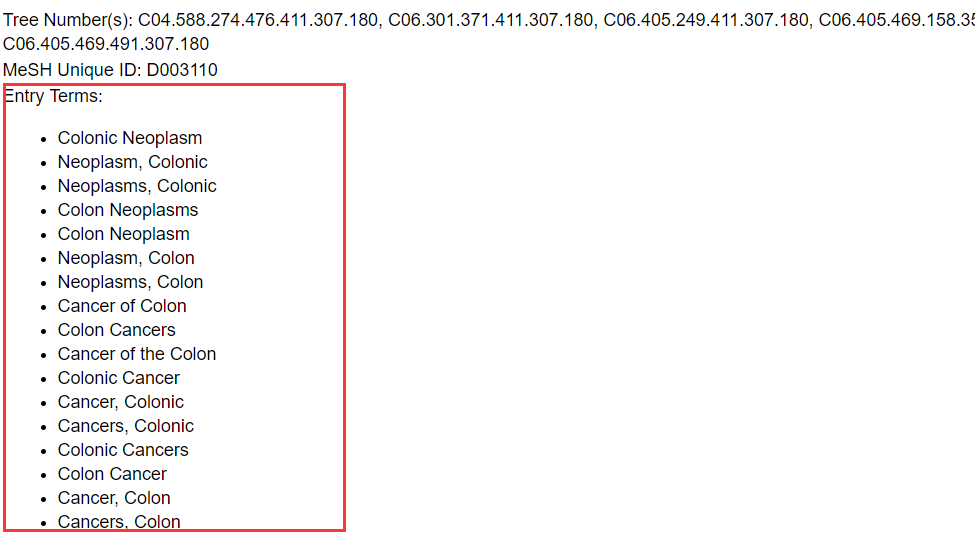
\includegraphics[width=0.4\linewidth]{查询扩展.png}
  \caption{查询扩展} 
  \label{fig:expansion}
  \vspace{1em}
\end{figure}

\subsection{检索模型}
\textbf{词频(TF)}词在文档中出现的频度。频度越高,权重越大。一个5次提到同一词的字段比一个只有1次提到的更相关。词频的计算方式如下:
\begin{equation}
    tf(t, d)=\sqrt{\text{frequency}}
\end{equation}

其中,frequencty是$t$在文档$d$中出现次数。

\textbf{逆文档频率(IDF)}词在集合所有文档里出现的频率。频次越高,权重越低。常用词如 and 或the对相关度贡献很少,因为它们在多数文档中都会出现,一些不常见词如 elastic 或 hippopotamus可以帮助我们快速缩小范围找到感兴趣的文档。逆向文档频率的计算公式如下:
\begin{equation}
    idf(t)=1+\log{\frac{\text{numDocs}}{\text{docFreq+1}}}
\end{equation}

\textbf{字段长度归一值(norm)} 字段越短,字段的权重 越高 。如果词出现在类似标题 title 这样的字段,要比它出现在内容 body 这样的字段中的相关度更高。字段长度的归一值公式如下:
\begin{equation}
    \text{norm}(d)=\frac{1}{\sqrt{\text{numTerms}}}
\end{equation}

\textbf{查询归一化因子(QueryNorm)}试图将查询 归一化 , 这样就能将两个不同的查询结果相比较。这个因子是在查询过程的最前面计算的,具体的计算依赖于具体查询,一个典型的实现如下:
\begin{equation}
    \text{queryNorm} = \frac{1}{\sqrt{\text{sumOfSquaredWeights}}}
\end{equation}

其中,sumOfSquaredWeights是查询里每个词的IDF的平方和。

\textbf{查询协调(coord)}协调因子(coord)可以为那些查询词包含度高的文档提供奖励,文档里出现的查询词越多,它越有机会成为好的匹配结果。协调因子将评分与文档里匹配词的数量相乘,然后除以查询里所有词的数量。协调因子能使包含所有三个词的文档比只包含两个词的文档评分要高出很多。

\textbf{实用评分函数(Practical Scoring Function)}ElasticSearch采用布尔模型(Boolean model)、词频/逆向文档频率(TF/IDF)、以及向量空间模型(Vector Space Model),然后将他们合并到单个包中来收集匹配文档和分数计算。

只要一个文档与查询匹配,ElasticSearch就会为查询计算分数,然后合并每个匹配术语的分数。这里使用的分数计算公式叫做 实用计分函数(practical scoring function)。公式如下:

\begin{equation}
    \begin{aligned}
        \text{score}(q, d)= &\text{queryNorm}(q)\cdot\text{coord}(q,d)\\
        &\cdot\sum_{t\in q}{[tf(t, d)\cdot idf(t)^2\cdot t.getBoost()\cdot\text{norm}(t,d)]}\\
    \end{aligned}
\end{equation}

本实验采用实用评分函数为查询和文档计算相似度程度。

\pagebreak
\section{文档重排}
当我们从ElasticSearch中检索到top-k个文档时,我们将其输送到深度匹配模型,获得新的排序。接下来这一部分将会详细介绍该模型。
\subsection{深度相关匹配模型}
深度相关匹配模型(DRMM)\cite{guo2016deep}是目前在ad-hoc检索表现较好的一个深度匹配模型,本文采用该模型来进行文档重排。

DRMM在查询词级采用联合深层架构,在查询词和文档词之间进行相关匹配的局部相互作用。首先基于词嵌入在查询和文档建立每对词之间的局部相互作用。对于每个查询词,将可变长度的局部相互作用转换为固定长度的匹配直方图。基于固定长度匹配直方图,使用前馈匹配网络来学习分层匹配模式,并为每个查询词生成匹配分数。最后,通过将来自每个查询词的分数与词门控网络计算聚集权重而生成总体匹配分数。模型架构如图\ref{fig:drmm}所示:

\begin{figure}[!htbp]\centering
  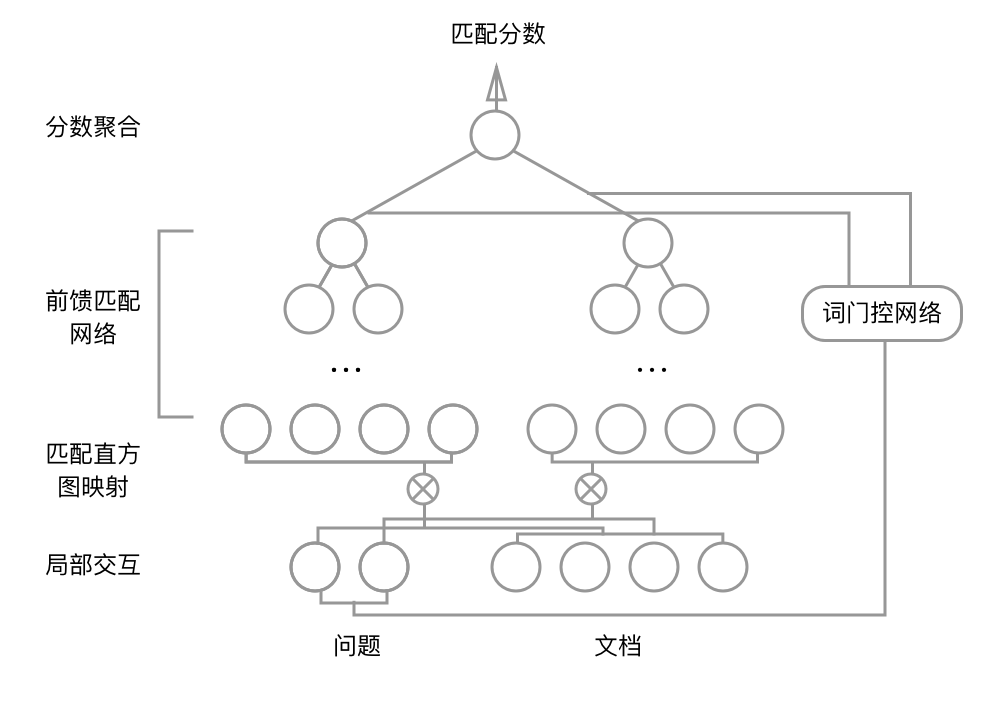
\includegraphics[width=0.9\linewidth]{DRMM.png}
  \caption{DRMM模型架构} 
  \label{fig:drmm}       % Give a unique label
  \vspace{1em}
\end{figure}

假设查询和文档表示为向量集$q=\{w_1^q, \cdots, w_M^q\}$和$d=\{w_1^d, \cdots, w_N^d\}$,其中,$w_i^q, i=1,\cdots, M, w_j^d, j=1, \cdots, N$表示为一个查询词向量和一个文档词向量。令$s$表示最终相关分数,则有:

\begin{equation}
    z_i^0=h(w_i^q\bigotimes d)
\end{equation}

\begin{equation}
    z_i^l=\tanh(W^lz_i^{l-1}+b^l)
\end{equation}

\begin{equation}
    s=\sum_{i=1}^Mg_iz_i^L
\end{equation}

其中$\bigotimes$表示查询词与文档词之间的相互作用算法,$h$表示从局部相互作用到匹配直方图的映射函数,$z_i^l$表示第$i$个查询词的中间隐藏层,$g_i$表示由词门控网络产生的聚合权重。$W^l$表示第$l$个权重矩阵,$b^l$表示第$l$个偏差项,它们在不同的查询词之间共享。该模型采用余弦相似度(cosine similarity)作为查询和文档每对词项之间的相互作用算子,使用已经存在的神经嵌入模型作为词向量。接下来,将详细描述该模型的主要组成部分,包括匹配直方图映射,前馈匹配网络和词门控网络。

\subsubsection{匹配直方图映射}

DRMM采用强度保留表示法,即匹配直方图,根据信号强度的不同等级而不是其位置对局部相互作用进行分组。具体而言,由于局部相互作用(即词向量之间的余弦相似性)处于区间[-1,1]之内,因此可以将区间离散为一组有序区段并累积每个区段中局部相互作用的计数。考虑固定区段大小并将精确匹配视为一个单独区段。例如,假设区段的大小设为0.5,我们将得到5个按升序排列的区段{[-1,-0.5),[-0.5,-0),[0,0.5),[0.5,1),[1,1]}。给定查询词“汽车”和文档(汽车,租赁,卡车,碰撞,禁令,跑道)以及基于余弦相似度的相应局部相互作用为(1,0.2,0.7,0.3,-0.1,0.1),将获得匹配的直方图为[0,1,3,1,1]。

\subsubsection{前馈匹配网络}

基于上述匹配直方图,DRMM模型使用前馈匹配网络来学习分层匹配模式,并为每个查询词生成匹配分数。
现有的以相互作用为中心的模型(例如MatchPyramid\cite{pang2016study})使用卷积神经网络来学习匹配矩阵上的分层匹配模式。这些模型基本上是利用具有局部“感受野”的卷积单元来进行位置感知,并在匹配模式中学习位置规律。这可能适用于图像识别任务,然而,它可能不适合问答任务。而该深度相关匹配模型旨在从不同层次的交互信号中提取分层匹配模式,而不是从不同的位置中提取。同时,由于匹配直方图直接区分精确匹配信号和其余部分,因此DRMM模型可以自然地学习到精确匹配信号的重要性。

\subsubsection{词门控网络}
DRMM模型与现有的以相互作用为中心的模型一个显着差异是在查询词级别采用了联合深度架构。通过这种方式,DRMM模型可以显式建模查询词的重要性。这是通过使用词门控网络来实现的,该网络为每个查询词产生聚合权重,控制该查询词上的相关性分值对最终相关性分值的贡献程度。具体而言,我们采用softmax函数作为门控函数:

\begin{equation}
    g_i=\frac{\exp(\omega_g\cdot x_i^q)}{\sum_j\exp(\omega_g\cdot x_j^q)}
\end{equation}

其中$\omega_g$表示词门控网络的权重向量,$x_i^q$表示第$i$个查询词的输入。词门控函数的输入为词向量。

\textbf{词向量(Term Vector,TV)}利用词嵌入来学习查询中的词权重,使用查询词向量作为词门控函数的输入。在这种方法中,$x_i^q$  表示第$i$ 个查询词向量,$\omega_g$  是具有和词向量相同维度的权重向量。
 
\pagebreak
\section{实验} 

\subsection{实验设置}

\subsubsection{数据预处理}

实验使用临床试验数据集(Clinical Trials dataset),有超过241006个xml文件。

我们将xml文件整理成csv文件,包括五个字段:查询id(qid),文档id(docid),查询文本(q\_text),文档文本(d\_text),文档排序(label)如表\ref{tab:csv}
\begin{table}[htbp]
\caption{数据格式}\label{tab:csv}
\centering
\begin{tabular}{ccccc}
\hline
qid & docid  & q\_text & d\_text & label \\
\hline
1 &	NCT00002455 &  query  & document & 0 \\
\hline
\end{tabular}
\end{table}


查询文本(query)来自topics2017.xml \footnote{http://www.trec-cds.org/topics2017.xml}如,每个查询包含4项:疾病类型disease,gene,demographic,other,我们使用了前三项,处理成字段名加内容,以空格连接,查询文本形式如下:

\begin{lstlisting}
disease Liposarcoma gene CDK4 Amplification age 38 gender male	
\end{lstlisting}

文档文本(document)来自xml\footnote{http://ClinicalTrials.gov},由于文档包含字段较多,我们选取了图\ref{fig:field}的13个字段来表示文档文本,处理成和查询文本同样的形式,字段名加内容,以空格连接。
\begin{figure}[!htbp]\centering
\vspace{1em}{}
  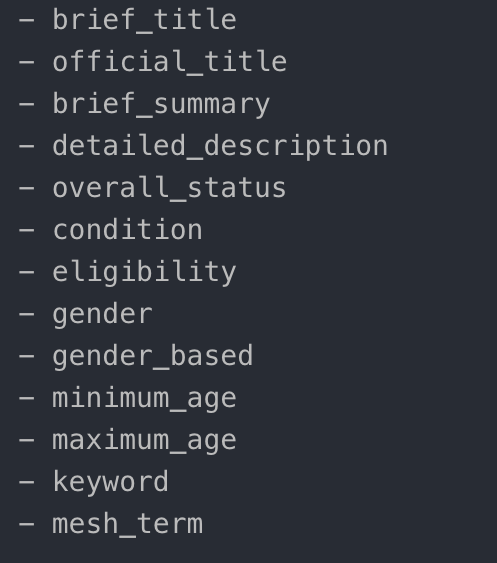
\includegraphics[width=0.4\linewidth]{选取字段.png}
  \caption{文档字段} 
  \label{fig:field}       % Give a unique label
  \vspace{1em}
\end{figure}
 \subsubsection{数据集划分}
本次实验中,我们采用五折交叉验证来划分数据集, 采用如下的话题(即查询)划分形式[28, 29, 25, 22, 6, 7], [26, 11, 1, 18, 21, 4], [19, 24, 27, 30, 12, 23], [13, 14, 3, 16, 8, 9], [15, 20, 5, 10, 17, 2] 。每一折中,使用3部分训练,1部分验证,1部分测试(即testset)报告模型的结果请对每一折的 test set 取平均.

\subsubsection{评价指标}
按照要求,我们采用$Precision@K$来评估检索模型的效果,如公式\eqref{precision}所示:
\begin{equation}
    \label{precision}
    Precision@K = \frac{tp@K}{K}
\end{equation}

其中,$tp@K$是前K个返回结果中真正例的数目,即被标识为相关的相关文档的数目。
在实验中,我们采用$Precision@5$,$Precision@10$和$Precision@15$来进行评估。

\subsubsection{DSL查询}
ElasticSearch的DSL查询如下所示:
\begin{lstlisting}[language=json,firstnumber=1]
{
    "query": {
        "bool": {
            "must": [{
                "multi_match": {
                    "query": disease,
                    "fields": ["brief_title^3", 
                               "brief_summary",
                               "detailed_description",
                               "condition",
                               "eligibility",
                               "keyword",
                               "mesh_term",
                               "official_title^2"],
                    "tie_breaker": 0.3,
                    "boost": 1.8
                }}, {
                "multi_match": {
                    "query": gene,
                    "fields": ["brief_title^3",
                               "brief_summary",
                               "detailed_description",
                               "condition",
                               "eligibility",
                               "keyword",
                               "mesh_term",
                               "official_title^2"],
                    "tie_breaker": 0.3
                }}
            ]
        }
    },
    "post_filter": {
        "term": {
            "gender": "all"
        }
    }
}
\end{lstlisting}

该查询表示在字段brief\_title、official\_title、brief\_summary、detailed-\_description、overall\_status、condition、eligibility、gender、gender\_based、minimum\_age、maximum\_age、keyword、mesh\_term中对disease和gene进行检索,其中brief\_title的权重设为3,official\_title的权重设为2,其余字段权重为1。计分方式为实用评分函数,最后整个文档的得分为相关度匹配最高的字段分数加上其他字段分数与tie\_breaker系数相乘的结果。即:
\begin{equation}
    Score = Score_{best field} + tie\_breaker \times \sum_{i \in other fields} Score_i
\end{equation}

同时,设disease的boost值为1.8,gene的boost为默认的1。

在查询的最后添加了对字段gender的后过滤,要求查询包含词“all”。

\subsubsection{参数设置}

\textbf{深度相关匹配模型(DRMM)} 
本实验采用铰链损失来训练DRMM。给定一个三元组$(q, d^+, d^-)$,其中对于查询$q$,文档$d^+$的排名高于文档$d^-$,损失函数定义为:
\begin{equation}
    \mathcal{L}(q,d^+,d^-;\theta)=\max(0, 1-s(q,d^+)+s(q,d^-))
\end{equation}

其中,$s(q,d)$表示$(q,d)$的预测匹配分数,$\theta$包括用于前馈匹配网络和用于词门控网络的参数。用于前馈匹配网络和用于词门控网络的参数。

我们在数据集上训练了word2vec\cite{mikolov2013distributed},并将之用于embedding layer的初始值。word2vec我们使用了gensim的实现,设置embedding的维数为300。优化器为Adam\cite{kingma2014adam},学习率设置为0.001,将训练数据分为32一组的小批量进行训练。


\subsection{实验结果}

% \begin{table}[htbp]
% \centering
% \caption{ElasticSearch、查询扩展和DRMM在测试集上的实验结果}\label{tab:results}
% \begin{tabular}{cclcclcclc}
% \hline
%              & \multicolumn{3}{c}{P@5}           & \multicolumn{3}{c}{P@10}          & \multicolumn{3}{c}{P@15}          \\ \hline
%              & ES              & EXP   & DRMM  & ES     & EXP   & DRMM           & ES     & EXP   & DRMM           \\ \hline
% CV0          & 0.3600          & 0.2400 & 0.3600 & 0.3600 & 0.2600 & 0.3600          & 0.2667 & 0.2267 & 0.3067          \\
% CV1          & 0.5333          & 0.5333 & 0.4333 & 0.4500 & 0.4833 & 0.4833          & 0.3667 & 0.3778 & 0.4000          \\
% CV2          & 0.4667          & 0.4667 & 0.4000 & 0.4167 & 0.4167 & 0.3667          & 0.3222 & 0.3444 & 0.3111          \\
% CV3          & 0.4333          & 0.4000 & 0.2667 & 0.3000 & 0.2667 & 0.3500          & 0.2222 & 0.1778 & 0.2889          \\
% CV4          & 0.3667          & 0.2667 & 0.4000 & 0.3833 & 0.2667 & 0.3833          & 0.3000 & 0.2111 & 0.3556          \\
% \textit{AVG} & \textbf{0.4320} & 0.3813 & 0.372  & 0.3820 & 0.3387 & \textbf{0.3887} & 0.2956 & 0.2676 & \textbf{0.3325} \\ \hline
% \end{tabular}
% \end{table}


\begin{table}[ht]
\centering
\caption{ElasticSearch、查询扩展、DRMM在测试集上的实验结果}\label{tab:results}
\begin{tabular}{cccccccc}\hline
                      &      & CV0    & CV1    & CV2    & CV3    & CV4    & AVG             \\ \hline
\multirow{3}{*}{P@5}  & ES   & 0.3600 & 0.5333 & 0.4667 & 0.4333 & 0.3667 & \textbf{0.4320} \\
                      & EXP  & 0.2400 & 0.5333 & 0.4667 & 0.4000 & 0.2667 & 0.3813          \\
                      & DRMM & 0.3600 & 0.4333 & 0.4000 & 0.2667 & 0.4000 & 0.3720          \\ \hline
\multirow{3}{*}{P@10} & ES   & 0.3600 & 0.4500 & 0.4167 & 0.3000 & 0.3833 & 0.3820          \\
                      & EXP  & 0.2600 & 0.4833 & 0.4167 & 0.2667 & 0.2667 & 0.3387          \\
                      & DRMM & 0.3600 & 0.4833 & 0.3667 & 0.3500 & 0.3833 & \textbf{0.3887} \\ \hline
\multirow{3}{*}{P@15} & ES   & 0.2667 & 0.3667 & 0.3222 & 0.2222 & 0.3000 & 0.2956          \\
                      & EXP  & 0.2267 & 0.3778 & 0.3444 & 0.1778 & 0.2111 & 0.2676          \\
                      & DRMM & 0.3067 & 0.4000 & 0.3111 & 0.2889 & 0.3556 & \textbf{0.3325}\\ \hline
\end{tabular}
\end{table}

ElasticSearch、查询扩展、DRMM在测试集上的实验结果如表\ref{tab:results}所示。其中,CV0、CV1、CV2、CV3、CV4表示交叉验证中的五折。ES表示原始查询经由ElasticSearch返回的结果;EXP表示原始查询经过扩展经由ElasticSearch返回的结果;DRMM表示将原始查询经由ElasticSearch返回的文档集输送到DRMM中重排后返回的结果。

从表\ref{tab:results}可以看出,ES和DRMM两个系统在测试集上表现较好,而EXP的效果较不理想。由于对DSL查询进行了精细化的定制,包括提升brief\_title,official\_title字段的重要性,对disease和gene予以不同的权重,并增加了对gender字段的后过滤,使得原始的查询在ElasticSearch上取得了不错的结果。而对于EXP,对disease进行同义词扩展之后,反而使得结果变差,这可能是由于增加后的查询变得过于复杂,返回的文档中噪声变多。DRMM虽然在P@10和P@15上有了小幅度的提升,但是这个效果并不让人满意。由于数据量本身较少且五折交叉验证,对于深度模型来说,难以学到数据的真实分布以及查询与文档之间的相关性。

\pagebreak
\section{代码及运行方法说明}
\subsection{代码及文件结构}
\begin{figure}[H]
	\centering
	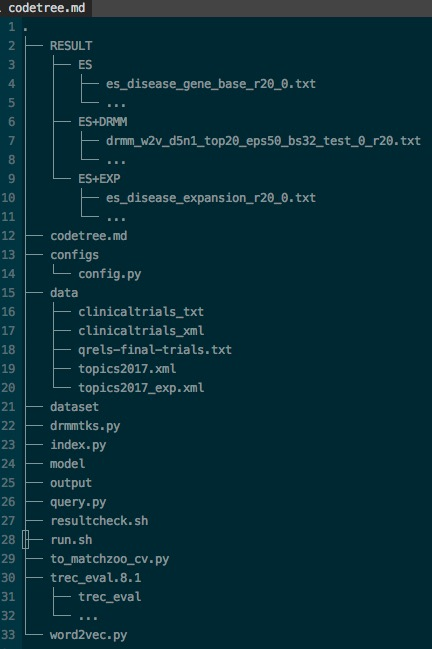
\includegraphics[width=0.7\linewidth]{5}
	\caption{代码及文件结构图}
	\label{fig:5}
\end{figure}
上图为本文的代码目录树形结构图。下面对目录结构中的文件及代码进行说明。
\par
\textbf{RESULT}文件夹下的文件为模型测试阶段生成的trec\_eval所需要的文件格式的所有结果。
\par
\textbf{codetree.md}中显示本组所实现的工程的目录结构。
\par
\textbf{configs}文件夹中的config.py为本工程的参数配置文件。
\par
\textbf{data}文件夹中存放的clinicaltrials.txt及clinicaltrials.xml为trec竞赛提供的病人病例数据库的snapshot,
topics2017.xml为所需要检索的30个主题的xml文件,
qrels-final-trials.txt为真实的所检索的主题与病人病例的相关性文件,
4个文件的下载页见\url{http://www.trec-cds.org/2017.html}, 
topics2017\_exp.xml为采用查询拓展后的检索文件。
\par
\textbf{dataset}文件夹下为采用5折交叉验证对数据集进行划分所形成的子数据集,并且子数据集已经格式化为本文所采用的深度匹配模型所需要的文件格式,对于第i(i=1,2,3,4,5)折划分,train\_i.csv为第i折数据的训练集,valid\_i.csv为第i折数据的验证集,test\_i.csv为第i折数据的测试集。
\par
\textbf{model}文件夹下的文件为保存的训练好后的模型。
\par
\textbf{output}文件夹下的文件为模型训练、验证、测试阶段生成的trec\_eval所需要的文件格式的所有结果。
\par
\textbf{trec\_eval.8.1}文件夹下包括我们运行结果检查时所需要的trec\_eval程序。
\par
\textbf{index.py}对病人数据库通过ElasticSearch建立索引,并且采用实用评分函数检索出TOP-K结果。
\par
\textbf{to\_matchzoo.py}对病人数据集采用5折交叉验证进行划分,并且将划分后的数据集格式化为深度匹配模型所需要的文件格式。
\par
\textbf{word2vec.py}采用词向量模型,将病人的文本数据转化为词向量表达。
\par
\textbf{drmmtks.py}对通过ElasticSearch检索出的TOP-K结果运用深度相关匹配模型DRMM进行重排序。
\par
\textbf{query.py}采用ElasticSearch模型以及采用深度匹配模型进行主题的检索,并输出trec\_eval所需要的文件格式的结果。
\par
\textbf{run.sh}为一键运行脚本,将index.py,to\_matchzoo.py,word2vec.py,drmmtks.py,query.py顺序封装,完成索引的构建,模型的训练,以及模型的测试。
\par
\textbf{resultcheck.sh}运行结果检查,输出测试集上的P@5,P@10,P@15结果。
\subsection{环境及依赖安装}
如需运行本文程序需要按照如下顺序安装本文所需的依赖模块。
本文python版本为3.6.4,Elasticsearch版本为6.5.4.

1.安装\textbf{numpy}(需使用最新版本)
\begin{verbatim}
    $ pip install numpy --upgrade
\end{verbatim}

2.安装hyperopt

目录下已经提供hyperopt安装包,执行以下命令:
\begin{verbatim}
    $ cd hyperopt-0.1.1
    $ python setup.py install
\end{verbatim}

3.安装深度匹配工具箱MatchZoo-2.0-dev

目录下已经提供Matchzoo解压缩后的安装包,执行以下命令:
\begin{verbatim}
    $ cd MatchZoo-2.0-dev
    $ python setup.py install
\end{verbatim}

4.安装nltk
\begin{verbatim}
    $ pip install nltk
\end{verbatim}

5.下载nltk停用词及punkt
\begin{verbatim}
    $ python
    >>> import nltk
    >>> nltk.download("stopwords")
    >>> nltk.download('punkt')
    >>> exit()
\end{verbatim}

6.安装JDK

根据系统下载安装所需的JDK\footnote{https://www.oracle.com/technetwork/java/javase/downloads/jdk8-downloads-2133151.html},并配置JAVA环境。

7.安装及运行Elasticsearch
\begin{verbatim}
    $ wget https://artifacts.elastic.co/downloads/elasticsearch/
    elasticsearch-6.5.4.tar.gz
    $ wget https://artifacts.elastic.co/downloads/elasticsearch/
    elasticsearch-6.5.4.tar.gz.sha512
    $ shasum -a 512 -c elasticsearch-6.5.4.tar.gz.sha512
    $ tar -xzf elasticsearch-6.5.4.tar.gz
    $ cd elasticsearch-6.5.4/
    $ $./bin/elasticsearch
\end{verbatim}

8.安装elasticsearch python module
\begin{verbatim}
    $ pip install elasticsearch
\end{verbatim}

\subsection{一键运行及结果检查界面}
一键运行命令:

\begin{verbatim}
    $ bash run.sh
\end{verbatim}
\par
\begin{figure}[H]
	\centering
	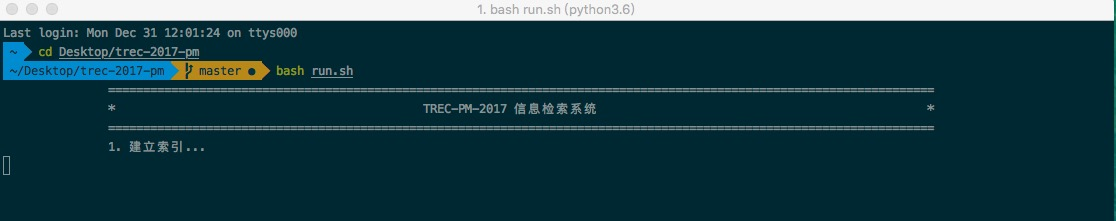
\includegraphics[width=0.7\linewidth]{4}
	\caption{一键运行程序}
	\label{fig:4}
\end{figure}
运行脚本前,请确认运行Elasticsearch,并且已将clinicaltrials.txt、clinicaltrials.xml、
topics2017.xml、qrels-final-trials.txt、topics2017\_exp.xml5个文件放在data文件夹下。
\par
运行该脚本,会顺序完成索引构建、模型训练、模型测试三个步骤,模型训练、验证、测试的结果均保存在output文件夹,我们将测试集结果提取到RESULT文件夹以进行结果检查。
\par
结果检查界面
\begin{verbatim}
    $ bash resultcheck.sh
\end{verbatim}
\par
进入界面后,界面上方显示三个模型的名称:0,Elasticsearch模型;1,Elasticsearch+查询扩展模型;2,Elasticsearch+深度相关匹配DRMM模型。
\par
界面中央展示了三个不同模型在五折测试集上的准确率P@5,P@10,P@15的均值,输入序号0,1,2可分别进入3个对应模型的结果检查子界面,输入e退出程序。
\begin{figure}[H]
	\centering
	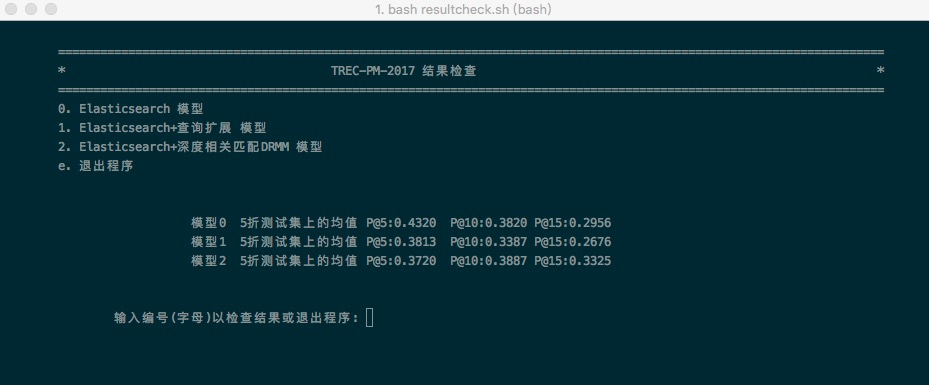
\includegraphics[width=0.7\linewidth]{1}
	\caption{结果检查界面}
	\label{fig:1}
\end{figure}
\par
下图7展示了Elasticsearch+深度相关匹配DRMM模型的结果检查界面,输入0,1,2,3,4可分别显示对应测试集的结果,输入b可返回上级目录。
\begin{figure}[H]
	\centering
	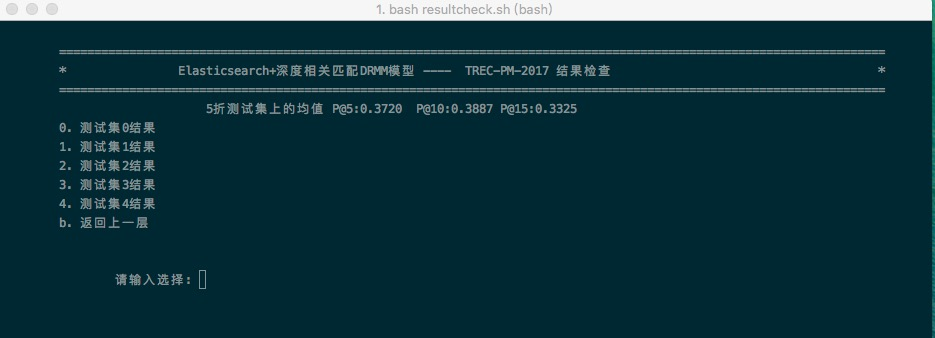
\includegraphics[width=0.7\linewidth]{2}
	\caption{ES+DRMM模型结果检查选择界面}
	\label{fig:2}
\end{figure}
\par 下图8展示了Elasticsearch+深度相关匹配DRMM模型在测试集0上的trec\_eval运行结果,按任意键可返回上级目录。
\begin{figure}[H]
	\centering
	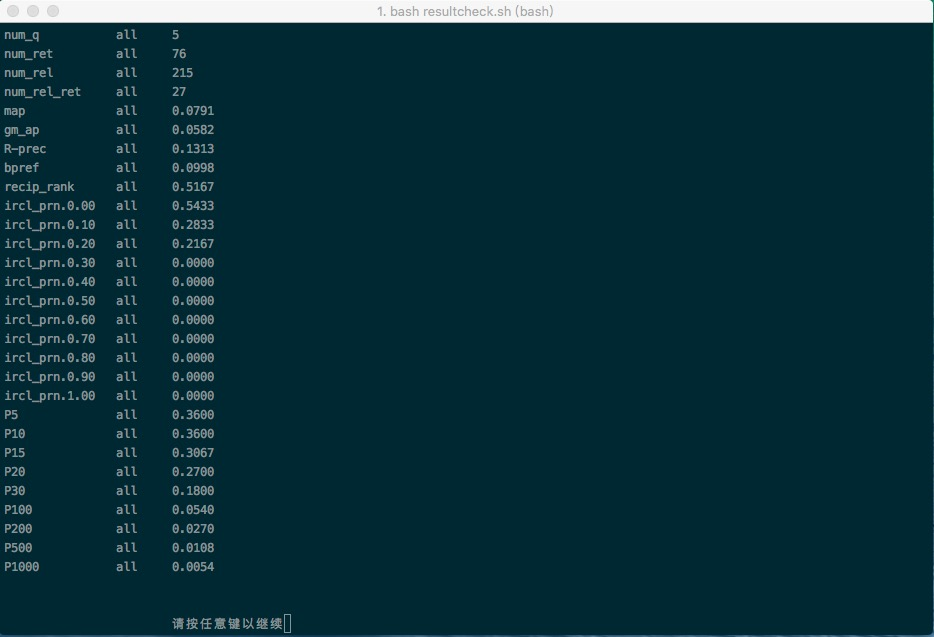
\includegraphics[width=0.7\linewidth]{3}
	\caption{ES+DRMM模型在测试集0上的trec\_eval运行结果图}
	\label{fig:3}
\end{figure}


\pagebreak
\section{总结及讨论}

对于许多复杂的疾病,没有针对特定诊断患者的“一刀切”解决方案。患者的正确治疗取决于遗传、环境和生活方式的选择。基于这些因素以科学严谨的方式个性化治疗的能力是新兴的“精准医疗”范式的标志。精准医疗对癌症治疗的潜在影响最为密切,在癌症中,针对特定患者的治疗完全基于患者肿瘤中的特定基因突变,对其他患者可能是有效的,甚至是致命的。

将精准医疗的发现付诸实践的一个根本难题是,从本质上讲,精准医疗创造了巨大的治疗选择空间。这很容易让那些试图了解最新情况的临床医师们感到头昏眼花,也很容易阻止临床医师为特定患者确定最佳治疗方案的尝试。然而,快速定位相关证据的能力是信息检索(IR)的标志。

本实验经过前期调研共设计并实现了三套方案。其中,基于ElasticSearch的无扩展查询取得了较好的效果,这说明在对查询进行精细化设计的基础上,传统模型依然具有强大的匹配能力。我们也探索了查询扩展对实验结果的影响,可能由于查询扩展后噪声的增多,效果反而变差。同时,由于数据量较少,使得深度模型在该数据集上的表现不佳,仅在P@10与P@15中有小幅度的提升。若有足够的数据集并且对短文本有更好的表示,深度模型可能会取得不俗的结果。

\clearpage
% -----------------------------------REFERENCE----------------------------------------
\bibliography{citation}
\addcontentsline{toc}{section}{参考文献}
\end{document}

